\begin{figure}[H]
\centering
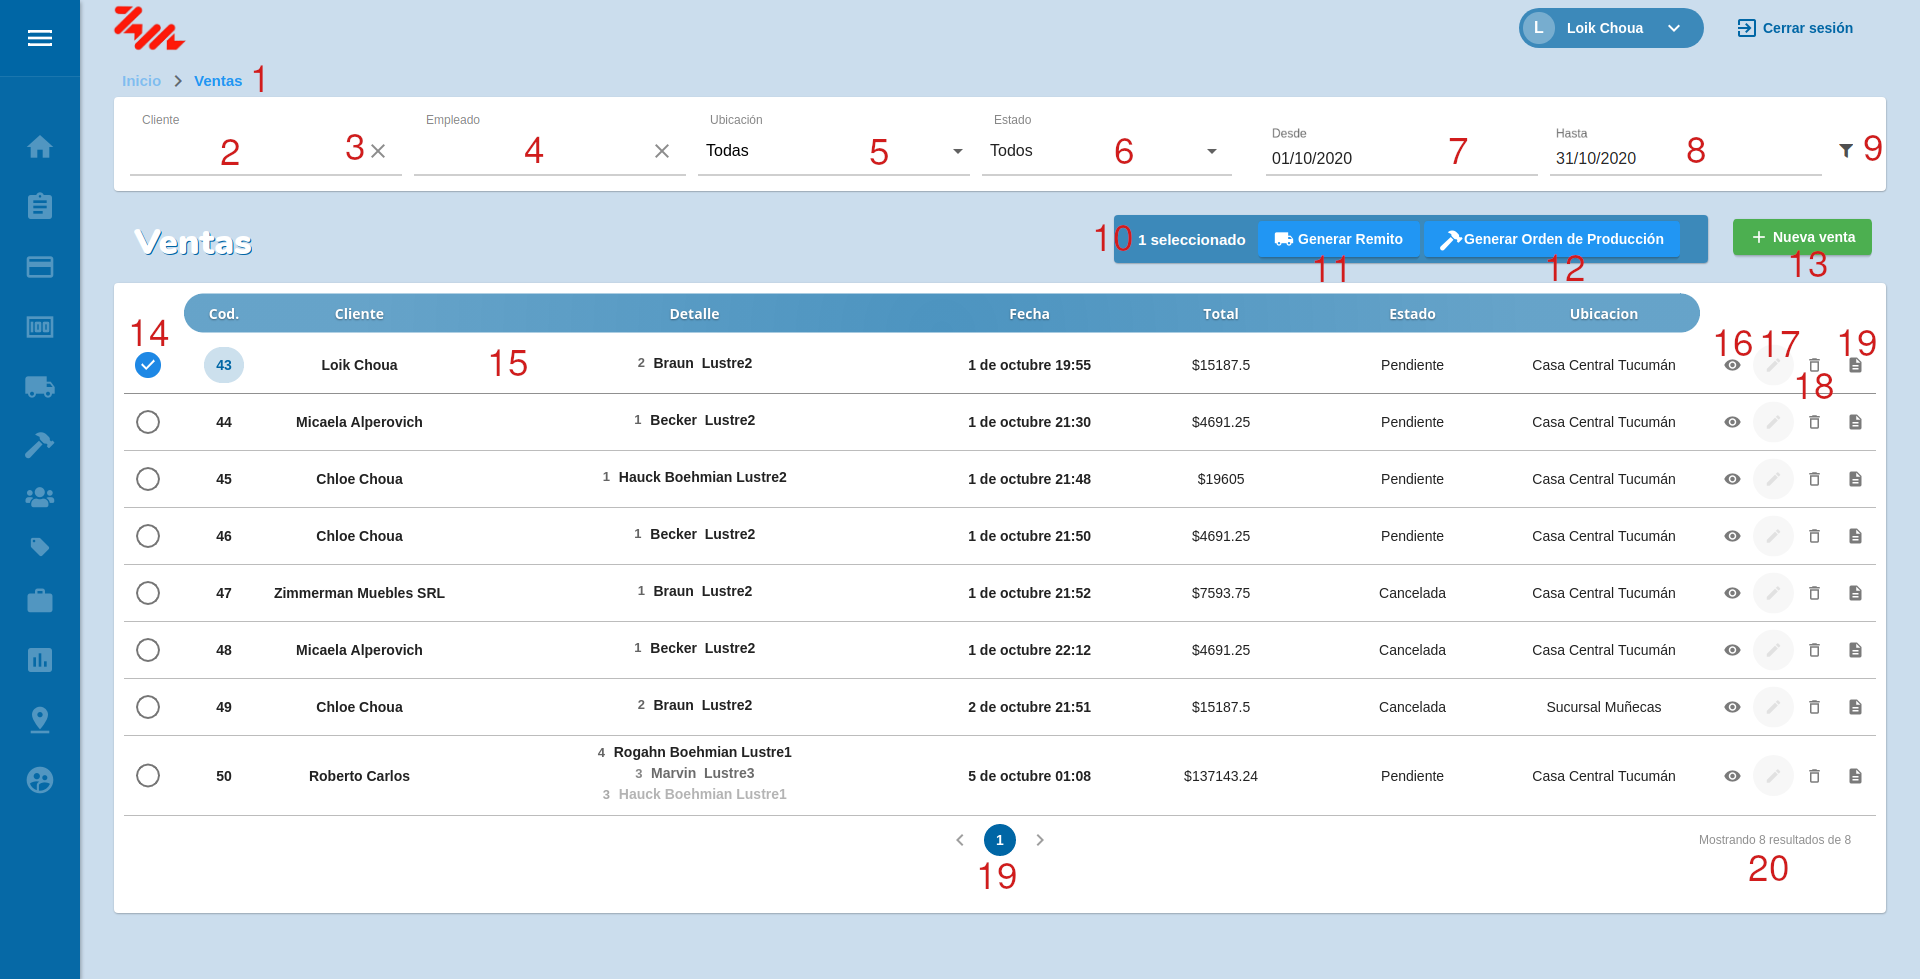
\includegraphics[width=\textwidth,height=\textheight,keepaspectratio]{Escenarios/AD-10-00}
\caption{Escenario - AD-10-00}
\label{fig:AD-10-00}
\end{figure}
Este escenario muestra toda la información referida a las ventas, junto con las acciones disponibles.
El botón \textbf{AD-10-01} permite navegar al escenario \textbf{AD-02-00}. El campo \textbf{AD-10-02} permite ingresar un cliente para filtrar las ventas por cliente, el campo cuenta con el botón \textbf{AD-03-03} que permite borrar el texto ingresado en el campo. El campo \textbf{AD-03-04} permite al usuario buscar ventas de acuerdo al empleado que la realizó. La lista desplegable \textbf{AD-10-05} permite filtrar de acuerdo a la ubicación en dónde se creó la venta. La lista desplegable \textbf{AD-10-06} permite al usuario filtrar por los estados en los cuales puede encontrarse la venta. Los campos  \textbf{AD-10-07} y \textbf{AD-10-08} permiten al usuario filtrar las ventas de acuerdo a un rango de fechas en la cual fueron creadas. El botón \textbf{AD-10-09} permite visualizar más filtros de búsqueda disponibles, como ser el producto, la tela y el lustre.
El campo \textbf{AD-10-10} se muestra cuando se ha seleccionado al menos una venta de la tabla, e indica la cantidad de ventas seleccionadas. El botón \textbf{AD-10-11} permite al usuario crear un remito a partir de la venta seleccionada y navega al escenario \textbf{AD-21-00}. El botón \textbf{AD-10-12} permite al usuario crear una órden de producción a partir de la venta seleccionada y navega al escenario \textbf{AD-23-00}. El botón \textbf{AD-10-13} permite al usuario crear una nueva venta y navega al escenario \textbf{AD-11-00}.
El botón \textbf{AD-10-14} permite al usuario seleccionar una o más ventas del resultado de la búsqueda. El campo \textbf{AD-10-15} muestra la información relacionada a las ventas especificando el código, el cliente , el detalle de venta, la fecha de creación, el total de la venta, el estado en el cúal se encuentra y la ubicación en el cual fue creado. El botón \textbf{AD-10-16} permite navegar al escenario \textbf{AD-12-00} para ver la venta, el botón \textbf{AD-10-17} permite al usuario editar la venta navegando al escenario \textbf{AD-11-00} y el botón \textbf{AD-03-18} permite al usuario borrar la venta. 
En  \textbf{AD-10-19} se mostrarán las páginas de resultado, pudiendo cambiar de página. En \textbf{AD-10-20} se mostrará cuantos resultados se están visualizando y el total.
\clearpage
